% Класс документов по ГОСТ 7.32-2001 "Отчёт о научно-исследовательской работе"
% на основе ГОСТ 2.105-95
% Автор - Алексей Томин, с помощью списка рассылки latex-gost-request@ice.ru,
%  "extreport.cls", "lastpage.sty" и конференции RU.TEX
% Лицензия GPL
% Все вопросы, замечания и пожелания сюда: mailto:alxt@yandex.ru
% Дальнейшая разработка и поддержка - Михаил Конник,
% связаться можно по адресу mydebianblog@gmail.com
% Подгонка проекта под реалии 17-й кафедры - Жаров Ярослав. 
% Связь через mart.slaaf@gmail.com или через github - MartSlaaf

\documentclass[utf8,usehyperref,14pt]{G7-32}
\usepackage[T2A]{fontenc}
\usepackage[utf8]{inputenc} %% ваша любимая кодировка здесь
\usepackage[english,russian]{babel} %% это необходимо для включения переносов
\usepackage{float}
\usepackage{graphicx} % работа с графикой
\usepackage{listings} % для возможности вставки исходников
\usepackage{cmap} % pdf должен быть копируемым, для проверки на цитирование
\graphicspath{{pictures/}}
\lstset{breaklines=true, language=R}
\TableInChaper % таблицы будут нумероваться в пределах р1аздела
\PicInChaper   % рисунки будут нумероваться в пределах раздела
\setlength\GostItemGap{2mm}% для красоты можно менять от 0мм

% Определяем заголовки для титульной страницы

\NirManager{}{Катаев Д.Е.} %% {научное звание и должность}{ФИО} - руководителя

%\NirYear{2014}%% если нужно поменять год отчёта; если закомментировано, ставится текущий год
\NirTown{Москва} %% город, в котором написан отчёт

\NirStudentGroup{K10-171} % группа
\NirStudent{Жаров Я.М.} % ФИО

\bibliographystyle{unsrt} %Стиль библиографических ссылок БибТеХа
%%%%%%%<------------- НАЧАЛО ДОКУМЕНТА
\begin{document}
\usefont{T2A}{ftm}{m}{} %%% Использование шрифтов Т2 для возможности скопировать текст из PDF-файлов.

\frontmatter %%% <-- это выключает нумерацию ВСЕГО; здесь начинаются ненумерованные главы типа Исполнители, Обозначения и прочее

\NirTitle{\textbf{«Модификация сверточной нейронной сети при помощи вейвлетов»}} % тема УИРа
%\DipTitle{\textbf{«Модификация сверточной нейронной сети при помощи вейвлетов»}} % тема Диплома

%\Referat
% Отчет \totalpages~с, \totaltables~таблица, \totalfigures~рисунок, \totalbibs~источник.

 \tableofcontents


\Introduction
В данное время распространена проблема распознавания образов и особенно оптических. Задача распознавания ставится в совершенно разных областях от распознавания маркировки или брака в изделиях на промышленных конвеерах, до распознавания рукописного текста при вводе на планшете. От распознавания узора сосудов на сетчатке глаза, или узоре папиллярного рисунка на пальцах до анализа состояния клеток крови. Увеличение автоматизации в данной области избавляет процесс распознавания от человеческого фактора, а повышение точности автоматических методов повышает скорость работы всего механизма. В области распознавания рукописного текста на данный момент лидирует метод сверточных нейронных сетей, предложенный в 1998 году Яном Лекуном. За время существования концепция сверточных нейронных сетей обрела не только славу передового метода в решении задачи распознавания образов, но и некоторое количество практических приложений \cite{microsoft_paper}. В данной дипломной работе описывается разработка, реализация и тестирование двух изменений в процесс обучения сверточной нейронной сети. В случае улучшения работы сети для данной работы, изначально являющейся экспериментом по продолжению темы предыдущих учебно-исследовательских работ в область распознавания оптических образов, может найтись так же практическое применение.

\mainmatter %% это включает нумерацию глав и секций в документе ниже
\chapter{Обзор методов и средств применимых для модификации сверточной нейронной сети при помощи вейвлетов}
\section{Постановка задачи модификации сверточной сети при помощи использования вейвлетов в слое свертки}
В данной работе проводилась попытка модификации сверточной нейронной сети архитектуры LeNet-5 методом замены ядер свертки, формируемых из отдельных связей, на ядра свертки, формируемые наложением вейвлетов. В оригинальной сверточной нейронной сети ядра свертки формируются из наборов настраиваемых весов. Например при образовании свертки размера $ 5 \times 5 $ используется 25 настраиваемых весов и, как правило, один дополнительный сдвиг. С помощью операции свертки уменьшается общее количество весов, так как возникает повторяемость использования веса. Например слой, который сворачивает изображение размером $ 32 \times 32 $ пикселов одной сверткой размером $ 5 \times 5 $ пикселов использует только 26 настраиваемых весов (25 весов на ядро свертки и один дополнительный вес для сдвига) и при этом имеет всего 20384 связи, вместо 803600 весов в случае полносвязного слоя (802816 для связей между слоями и 784 для сдвига). То есть уменьшает количество настраиваемых весов в 784 раза. Модификация, предлагаемая в данной работе позволяет заменить 26 настраиваемых параметров на 7-8, что позволяет еще раз сократить количество обучаемых параметров, хотя и не настолько же сильно, насколько переход от полносвязного слоя к сверточному. Методы распознавания изображений основанные на вейвлетахуспешно используются для распознавания лиц \cite{ViolaJones, YEF}.
\section{Сверточные нейронные сети}
Сверточные нейронные сети - архитектура нейронных сетей предложенная Яном Лекуном для распознавания изображений. Архитектура сверточных нейронных сетей основана на особенностях биологического зрения. В подражание простым клеткам в зрительной коре, которые реагируют на примитивы в считываемом с сетчатки изображении (например разнообразные наклонные линии), был создан сверточный слой сети. Сверточный слой содержит набор матриц, которые используются как ядра свертки. Когда на вход поступает раздражитель (изображение), сверточный слой проходит по нему сверточным фильтром, используя матрицы как ядра. Результат свертки используется как выходной сигнал слоя. Сверточные слои чередуются со слоями подвыборки, которые уменьшая количество пикселей улучшают обобщающую способность сети.\ref{CNN_arch} В некоторых случаях на выходе сети, для обработки результатов ставят персептрон. На данный момент сверточная нейронная сеть - подход показавший один из лучших результатов в классификации изображений.

\begin{figure}[H]
 \centering{
 	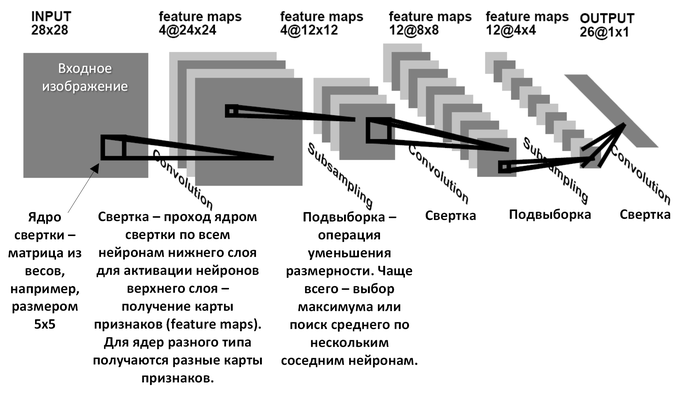
\includegraphics[width=0.75\textwidth]{convonet.png}
  }
  \caption{Типовая архитектура сверточной нейронной сети}\label{CNN_arch}
\end{figure}

\section{Алгоритм обучения backpropagation}
Алгоритм обучения методом обратного распространения ошибки - итеративный градиентный алгоритм для обучения многослойного персептрона. В общем смысле он заключается в распространении ошибки навстречу прямому распространению сигналов по сети и постоянной подстройке весов сети. При каждом обратном распространении веса в сети изменяются в направлении противоположном градиенту ошибки. С помощью итеративного повторения прямого и обратного распространения можно настроить сеть достаточно точно. 
Если принять, что $E(Z(t), Z'(t))$ - функция ошибки зависящая от $ Z(t) $ - выхода сети на шаге t и $ Z'(t) $ - предполагаемое значение выха сети, а так же ошибка - функция зависящая от весов сети $ \{w_{ij}\} $ то движение весов в общем случае следует осуществлять по следующей формуле:
\begin{equation}
\Delta w_{ij} = - \eta \frac{\partial E}{\partial w_{ij}}
\end{equation}

Если учесть что вес влият только на ту часть выход из слоя, с которой он соединен, то можно записать $ S_{j} = \sum_{i} w_{ij}x_{i} $. Используя правило взяти сложных производных можем записать следующее уравнение:
\begin{equation}
\frac{\partial E}{\partial w_{ij}} = \frac{\partial E}{\partial S_{j}}\frac{\partial S_{j}}{\partial w_{ij}} = x_{i}\frac{\partial E}{\partial S_{j}}
\end{equation}

Так как в свою очередь 
\begin{equation}
\frac{\partial E}{\partial S_{j}} = \frac{\partial E}{\partial o_{j}}\frac{\partial o_{j}}{\partial S_{j}} = \frac{\partial E}{\partial o_{j}}\frac{\partial \phi(S_{j})}{\partial S_{j}}, 
\end{equation}
  \begin{eqrem}
   & $ o_{j} $~--- выход слоя \\
   & $ \phi $~--- активационная функция нейрона \\
  \end{eqrem} \\
Отсюда очевидно возникает требование дифференциируемости активационной функции, что накладывает заметные ограничения на работу этого алгоритма.
Далее для любого слоя можно записывать формулу следующего вида:
\begin{equation}
\frac{\partial E}{\partial S_{j}} = \sum_{k \in outputs(j)}\frac{\partial E}{\partial S_{k}}\frac{\partial S_{k}}{\partial S_{j}}
\end{equation}
В данном случае сумма считается для всех выходов данного j-го элемента.
Вторая часть этого выражения вычисляется следующим образом:
\begin{equation}
\frac{\partial S_{k}}{\partial S_{j}} = \frac{\partial S_{k}}{\partial o_{j}}\frac{\partial o_{j}}{\partial S_{j}} = w_{ij}\frac{\partial \phi(S_{j})}{\partial S_{j}}, 
\end{equation}
а выражение $ \frac{\partial E}{\partial S_{k}} $ - поправка вычисленная для узла следующего слоя. Таким цепным образом вычисляется ошибка, для обратного распространения.

К данному алгоритму часто применяют разнообразные оптимизации, такие, как например алгоритм Левенберга-Марквардта \cite{LM}. При своей популярности алгоритм имеет некоторые проблемные места, для данной работы ключевой проблемой было требование к дифференциируемости передаточной функции.

\section{Алгоритм обучения ALOPEX}
ALOPEX (ALgorithm fOr Pattern EXtraction), это алгоритм обучения основанный на корреляции изменений в весах и изменением оценочной функции. Допустим мы ищем минимум некоторой функции $ f(x_{1}, x_{2}, … ,x_{n}) $. В таком случае если мы $ f(x_{1}-a, x_{2}, … ,x_{n}) <  f(x_{1}, x_{2}, … ,x_{n}) $, то на следущей итерации следует положить $ x_{1} = x_{1}-a $ и продолжить исследование. Если записать данный алгоритм для весов, получим:
\begin{equation}
w_{ij}(n) = w_{ij}(n-1) + \delta_{ij}(n)
\label{main_alopex}
\end{equation}
, где $ \delta $ это коэффициент, зависящий от корреляции между оценочной функцией и предыдущим изменением веса, вычисляемый по следующей формуле:
\begin{equation}
\delta_{ij}(n) = \eta * sgn(u - p_{ij}(n)) 
\end{equation}
В данном случае u - случайная переменная равномерно распределенная на отрезке $ (0, 1) $, $\eta$ - коэффициент обучения, а $ p_{ij} $ зависит от движений оценочной функции и данного веса следующим образом:
\begin{equation}
p_{ij}(n) = \phi (\Delta w_{ij}(n) * \Delta E_{ij}(n) / T(n)), 
\end{equation}
где $ \phi $ - логистическая сигмоида, $ \Delta x(n) = x(n-1) - x(n-2) $, а T - температурный коэффициент он играет ту же роль, что и температура, в случае имитации отжига. Он может модифицироваться как по линейному закону, так и по более усложненным правилам. Например наиболее простым является такое правило, применяемо каждые N шагов:
\begin{equation}
T(n) = \frac{1}{NM} \sum_i \sum_j \sum_{n'=n-N}^{n-1} |\Delta w_{ij}(n') * \Delta E_{ij}(n')|
\label{alopex_annealing}
\end{equation}
Если использовать для всех весов одинаковый коэффициент обучения, формулу можно сократить до:
\begin{equation}
T(n) = \frac{\eta}{N} \sum_{n'=n-N}^{n-1} |\Delta E_{ij}(n')|
\end{equation}
Существует однако формула позволяющая ускорить сходимость такого алгоритма. Такая модификация назвается ALOPEX-B\cite{carlo_alopex}. В данном случае отличается  вычисление $ p_{ij}$. Оно становится следующим:

\begin{equation}
p_{ij}(n) =\phi ( \frac{sgn(\Delta w_{ij}(n)) \Delta E_{ij}(n)}{\sum_{k=2}^{n} \lambda (\lambda-1)^{n-k}|\Delta E_{ij}(k-1)|})
\end{equation}

А так же общую формулу \eqref{main_alopex} следует заменить на 

\begin{equation}
w_{ij}(n) = w_{ij}(n-1) + \delta_{ij}(n) + \gamma \Delta w_{ij}(n) \Delta E_{ij}(n)
\end{equation}

Основным преимуществом алгоритма ALOPEX является отсутствие требования к наличию производной и к самой возможности ее взятия. Есть множество разнообразных модификаций этого алгоритма, таких как, например, ALOPEX основанный на методе Монте-Карло\cite{carlo_alopex}. Однако большинство модификаций достаточно сложны в реализации, и приносят недостаточно большой выигрыш. В данной работе использовался простой ALOPEX алгоритм с T вычисляемым по формуле \eqref{alopex_annealing}, так как основной задачей было проверить работоспособность спроектированной модификации.

\section{Архитектура сверточной нейронной сети LeNet-5}
В данной работе использовалась архитектура сети LeNet-5, предложенная Яном Лекуном \cite{LeCun}. Эта сеть характеризуется одной из наибольших скоростей обучения, и одними из лучших результатов в распознавании рукописных цифр.
LeNet-5 состоит из 7 слоев, каждый из которых содержит обучаемые веса.
\begin{itemize}
\item Первый слой принимает на вход изображение размером $ 32 \times 32 $ пиксела и проводит свертку при помощи 6 ядер размером $ 5 \times 5 $ пикселов. Первый слой содержит 156 обучаемых параметров и 122304 связи. На выходе получается изображение размером $ 28 \times 28 $ пикселов.
\item Второй слой проводит процедуру прореживания изображения с маской размером $ 2 \times 2 $ пиксела. После суммирования пикселов в маске значение умножается на настраиваемый вес и суммируется с настраиваемым коэффициентом сдвига. Данный слой содержит 12 настраиваемых параметров и 5880 связей. На выходе получается изображение размером $ 14 \times 14 $ пикселов.Этот слой содержит 1516 настраиваемых параметров и 151600 связей. На выходе из данного слоя получается изображение размером $ 10 \times 10 $ пикселов.
\item Третий слой проводит свертку с помощью 16 ядер размером $ 5 \times 5 $. Свертки проводятся группами, после чего результаты для одного ядра усредняются. Каждое ядро применяется к разным наборам слоев, по следующей схеме 

\[ \begin{array}{c|cccccccccccccccc}
   & 0 & 1 & 2 & 3 & 4 & 5 & 6 & 7 & 8 & 9 & 10 & 11 & 12 & 13 & 14 & 15\\ \hline
 0 & X &   &   &   & X & X & X &   &   & X & X & X & X &   & X & X \\
 1 & X & X &   &   &   & X & X & X &   &   & X & X & X & X &   & X \\
 2 & X & X & X &   &   &   & X & X & X &   &   & X &   & X & X & X \\ 
 3 &   & X & X & X &   &   & X & X & X & X &   &   & X &   & X & X  \\ 
 4 &   &   & X & X & X &   &   & X & X & X & X &   & X & X &   & X \\ 
 5 &   &   &   & X & X & X &   &   & X & X & X & X &   & X & X & X \end{array} \]


\item Четвертый слой проводит прореживание изображения по аналогии со вторым слоем. В данном случае так же используются настраиваемые веса и сдвиги. Слой содержит 32 настраиваемых параметра и 2000 связей. на выходе получаются карты признаков размером $ 5 \times 5 $ пикселов.
\item Пятый слой проводит свертку всех 16 карт признаков полученных от предыдущего слоя 120 ядрами размера $ 5 \times 5 $ пикселов. Каждое ядро применяется ко всем входным картам и результат усредняется. На выходе получается 120 изображений состоящих из одного пиксела. В дальнейшем этот выход можно интерпретировать как вектор признаков изображения. Этот слой содержит 48120 настраиваемых весов и столько же связей. На выходе получаем вектор из 120 признаков.
\item Шестой слой является полносвязным слоем принимающим на вход 120 значений и выдающим на выходе 84 значения. В данном слое содержится 10164 настраиваемых веса. Это классический полносвязный слой в котором в качестве активационной функции используется сигмоида.
\item Седьмой слой представляет из себя слой с радиально-базисной активационной функцией. Общий вид функции $ y_{i} = \sum_{j}(x_{i} - w_{ij})^2 $ на выходе имеет вектор признаков размерности 10. В данном векторе каждой цифре соответствует отдельный элемент. Элемент с наибольшим значением считается наиболее вероятным результатом распознавания.
\end{itemize}
При обучении сети данной архитектуры используется алгоритм обратного распространения ошибки. Обучение происходит пакетами размером в 10 изображений, то есть веса исправляются не после каждого прямого распространения, а по результатам 10 прямых распространений. 
Популярные различные модификации алгоритма обучения например алгоритм Левенберга-Марквардта. В данной работе использовалась библиотека с реализованным алгоритмом Левенберга-Марквардта.

\section{Прицнипы и причины оценки библиотек с открытым исходным кодом и реализующих сверточные нейронные сети}
Для реализации практической части диплома было принято решение использовать и модифицировать готовую библиотеку реализующую механизм сверточной нейронной сети. Модификация вместо реализации своими силами была выбрана по следующему набору причин:
\begin{enumerate}
\item Возможность серьезно сократить время реализации, тем самым получив больше времени на разработку и проведение экспериментов;
\item Возможность сравнить результаты и время работы модификации и исходной сети в наиболее близких условиях;
\item Возможность получить значительно более быструю реализацию, чем та, которую позволяли бы реализовать текущие навыки.
\end{enumerate}
Исходя из такого списка причин был составлен основной список параметров по которым велось сравнение библиотек:
\begin{enumerate}
\item Модульная система инициализации нейросети. Подобная система реализации позволяет заменить конкретный модуль нейросети своим и, практически не изменяя остальных, использовать готовое решение.
\item Поддержка открытым сообществом или одиночным открытым разработчиком, что потенциально повышает шансы на получение помощи от разработчика или сообщества, при возникновении сложной ситуации в процессе разработки.
\item Актуальная поддержка. Постоянное обновление исходного кода библиотеки позволяет оценить скорость устранения проблем, при наличии таковых.
\end{enumerate}
Список библиотек, подвергнутых сравнению:
ConvNet, EBlearn, cuda-convnet, nnForge, encog and tiny-cnn.

\section{Результаты сравнения библиотек с открытым исходным кодом и реализующих сверточные нейронные сети}
\begin{enumerate}
\item Проект ConvNet, не смотря на наличие некоторой популярности и сообщество пользователей так и не вышел из стадии пре-альфа версии. При этом прекратил поддержку автором примерно в 2008 году. Так же в данном проекте остался нереализованным механизм обучения, что так же ставит под сомнение возможность использования данной сети для ускорения реализации дипломного проекта.
\item EBlearn. Эта библиотека наиболее близка к оригинальной идее, так как один из ее разработчиков и руководителей - Ян ЛеКун, являющийся автором идеи сверточных нейронных сетей. Так же эта библиотека активно развивается, и последнее серьезное обновление вышло менее двух лет назад. Однако библиотека в силу практического использования и множества разносторонних применений имеет весьма масштабную структуру \ref{eblearn}, с которой, возможно, будет тяжело справиться.
\begin{figure}[h]
 \centering{
 	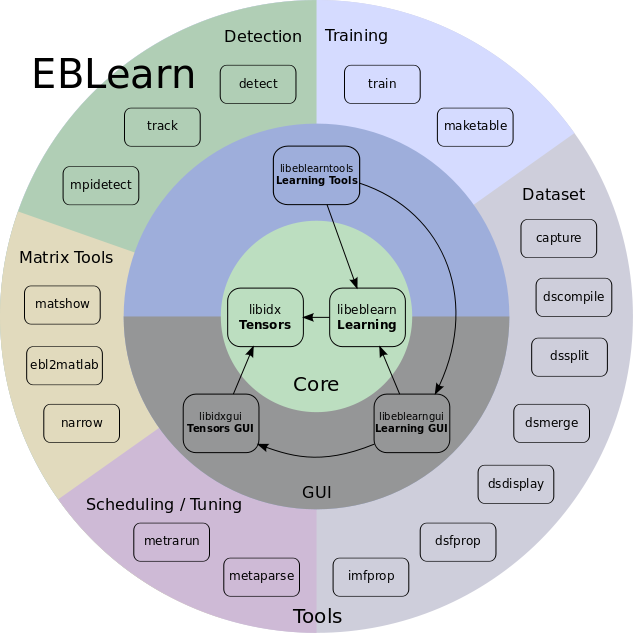
\includegraphics[width=0.75\textwidth]{eblearn.png}
  }
  \caption{Общая архитектура библиотеки EBlearn}\label{eblearn}
\end{figure}
\item Библиотека tiny-cnn развивается практически одиночным разработчиком, однако достаточно регулярно обновляется (последнее около полугода назад), имеет простую структуру (в частности в силу того, что не ставит своей целью ничего, кроме реализации сверточных нейронных сетей) и язык реализации С++. Что позволяет без проблем редактировать исходный код. Так же данная библиотека обладает модульной системой инициализации.
\item Cuda-convnet ставит основной целью реализацию быстрой работы сверточных нейронных сетей на при помощи вычисления на графических процессорах. В данном случае это не могло являться серьезным плюсом, в силу отсутствия у меня требуемого для этих целей оборудования и возможности его быстро получить. Однако, данная библиотека активно развивается и позволяет достаточно легко менять типы нейронов. Вероятно эта библиотека будет использована при реализации линейной вариации использования вейвлетов в сверточной нейронной сети.
\item nnForge является наиболее активно развивающейся из всех приведенных библиотек, на момент написания время с последнего обновления состовляет меньше недели. Так же язык разработки С++ и активное сообщество создающееся вокруг данного проекта позволяет надеятся на возможность помощи. Модульная система слоев позволяет модифицировать исключительно отдельный слой.
\end{enumerate}


\section{Результаты оценки}
В результате оценки разнообразных библиотек на тему соответствия критериям как финальные библиотеки, на основе которых будет производиться реализация были выбраны библиотеки nnForge и tiny-cnn. Эти библиотеки выбирались исходя из весьма специфических требований, поэтому не удивительно, что в список выбранных библиотек не вошли наиболее популярные библиотеки. Основной целью была легкость модификации, а не простота финального использования. Так как основная цель - оценить работоспособность соответствующего подхода модификации сверточных нейронных сетей.

\section{Библиотека для использования в ходе модификаций}
Так как подробный анализ и выбор производился выше, следует описать причины выбора данной библиотеки и ее особенности.
Библиотека tiny-cnn  была выбрана из множества претендентов по следующему набору параметров:
\begin{enumerate}
\item Базовая скорость работы. Библиотека обладает достаточно высокой скоростью работы без необходимости длительной настройки для конкретного рабочего компьютера. Для ускорения работы в библиотеке широко использовались средства библиотек Boost,  Intel TBB и OMP.
\item Поддержка. Данная библиотека продолжает поддерживаться на данный момент. Прямо в ходе внесения изменений была возможность консультироваться с создателем библиотеки и получать исправления.
\item Баланс между оптимизацией и читаемостью. В библиотеке соблюдена визуальная чистота и мнемоничность кода, что позволило достаточно легко вносить изменения в код библиотеки.
\item Широта разработанных методов. В данной библиотеке были реализованы как базовые методы обучения, так и, например, метод Левенберга-Марквардта. 
\end{enumerate}

Данная библиотека реализована в заголовках, что позволяет просто подключать ее к любому проекту. После включения заголовочных файлов становится доступно пространство имен со всем функционалом. Основным абстрактным классом является класс слоя, подобная модульная структура позволяет легко дополнять код библиотеки новыми видами слоев, для реализации различного функционала. Еще одним ключевым абстрактным классом является класс оптимизаторов - от этого класса наследуются все механизмы занимающиеся настройкой весов. Класс оптимизатор собирается вместе с набором экземпляров слоев в экземпляр сети. Пример абстрактного класса слоя находится в приложении \ref{abslayer}. Как можно видеть из этого кода библиотечные классы реализованы достаточно подробно, читаемо и с высокой степенью наследования.

\chapter{Разработка и реализация модификаций}
В данной работе предлагается два изменения вводимых в сверточную нейронную сеть. Первое из этих изменений относится к изменению процесса инициализации сверточных слоев сети, второе относится к изменению как процесса инициализации, так и к изменению процесса обучения сети.

\section{Конструирование ядра свертки из вейвлетов}
Сборку ядра свертки из вейвлетов можно разделить на следующие шаги:
\begin{enumerate}
\item Инициализируем ядро свертки размера $ n \times n $ нулевыми значениями
\item Инициализируем набор из $ k $ двумерных вейвлетов хаара, для каждого из которых случайным образом выбираются:
\begin{itemize}
\item координаты начала $X, Y : 0 \leq X, Y < n$;
\item поворот: вдоль вертикальной или горизонтальной оси $R \in (x, y)$;
\item размер вдоль выбранной оси $ S: 1 \leq S \leq n $;
\item коэффициент влияния $ Z \in [-1, 1] $ - то есть множитель на который домножается собственно вейвлет-функция;
\end{itemize}
\item для каждого вейвлета из принадлежащих данному ядру обойти все элементы матрицы и добавить к ним значение вейвлета умноженное на значение коэффициента влияния
\end{enumerate}

\section{Изменения в инициализации сверточного слоя сети}
Данное изменение вносит минимальные помехи в обычную работу сверточной нейронной сети, поэтому может быть за минимальное время реализовано в большинстве библиотек предлагающих соответствующий функционал. В данном изменении предлагается инициализировать ядра свертки в сети не случайным набором чисел, а случайным набором двумерных вейвлетов Хаара \cite{chui, wavelet}. После инициализации сеть обучается по обычному алгоритму. Предполагается, что данное изменение может ускорить обучение сети на начальном этапе. Ускорение обучения на начальном этапе может быть актуально в том случае, когда, в силу непреодолимых условий, обучение занимает длительное время. В результате такого изменения сеть может обучиться лучше инициализированной случайно (при коротком времени) или не хуже (на длительном интервале).

\section{Изменения в процессе обучения сети}
Данное изменение вносит достаточно большое количество изменений в работу сверточной нейронной сети, и для его реализации требуется внести большое количество изменений в функционал большинства библиотек.  При данном изменении на каждом шаге обучения настраиваются веса конкретных вейвлетов, таким образом ядро свертки, конструируемое из них так же изменяется.
В архитектуре такого сверточного слоя происходит несколько изменений:
\begin{enumerate}
\item Для сверточного слоя имеет смысл хранить набор настроек вейвлетов. То есть для каждого ядра свертки каждого слоя должен храниться набор векторов {X, Y, R, S, Z}.
\item Обучаемым параметром сверточного слоя такого типа являются веса вейвлетов (Z). При смене знака вейвлет так же меняет направление, что позволяет оставить и этот параметр настраиваемым, при этом не вводя дополнительной переменной, и не устанавливая сложных правил для ее обучения.
\item В целях повышения быстродействия возможно хранение ядра свертки в собранном виде. Это позволяет не вычислять его каждый раз при прямом распространении. Соответственно конструирование ядра свертки происходит не по запросу, а каждый раз при подстройке весов
\end{enumerate}

В процессе обучения сети так же происходят изменения.
\begin{enumerate}
\item Так как применение в данном случае алгоритма обратного распространения ошибки затруднительно была сделана попытка применения алгоритма ALOPEX для обучения данного вида сети. В данной работе использовался алгоритм без использования коэффициента забывания, но с использованием температурного коэффициента 
\item В качестве функции оценки было выбрано количество правильных распознававаний  в пакете. Такая функция возможна при обучении пакетами, так как не требуется постоянной подстройки весов.
\item Обучение производилось пакетами по 100 изображений. Это позволяло более качественно оценить количество распознанных изображений. Так как при много меньшем размере пакета количество распознанных изображений могло сильно зависеть от изображений попавших в пакет, а в случае сильно увеличенного пакета количество подстроек весов в ходе одной эпохи падало, что сильно замедляло обучение.
\end{enumerate}

\section{Реализация изменения инициализации сети}
В случае данного изменения потребовались минимальные изменения. Был создан дополнительный класс для реализации соответствующего поведения. Единственным перегружаемым методом стал метод прямого распространения, так как инициализация весов была расположена гораздо глубже. Метод проверял инициализированы ли слои, если слои неинициализированы, проводилось конструирование матриц свертки из набора случайных вейвлетов, в противном случае управление передавалось в родительский метод прямого распространения. Пример кода находится в приложении \ref{matinit}.

\section{Реализация изменения обучения сети}
В данном случае пришлось создать целую структуру классов, повторяющую часть структуры обычных классов, для реализации алгоритма ALOPEX. На приведенной на рисунке диаграмме классов симметрично расположенные классы дублируют функционал с точностью до ориентированности на алгоритм ALOPEX. Слева от базового класса расположены элементы, которые были реализованы в библиотеке. Справа расположены элементы, которые были реализованы лишь при внесении модификации. Позже, для проверки работоспособности разных элементов алгоритма ALOPEX реализовывались отдельные скрипты для выполнения тестов. Побочным результатом данного этапа разработки можно считать дополнение кода библиотеки такими слоями как, например, слой вейвлонов. Что может использоваться в дальнейшем, при работе с вейвнетами.
\begin{figure}[H]
 \centering{
 	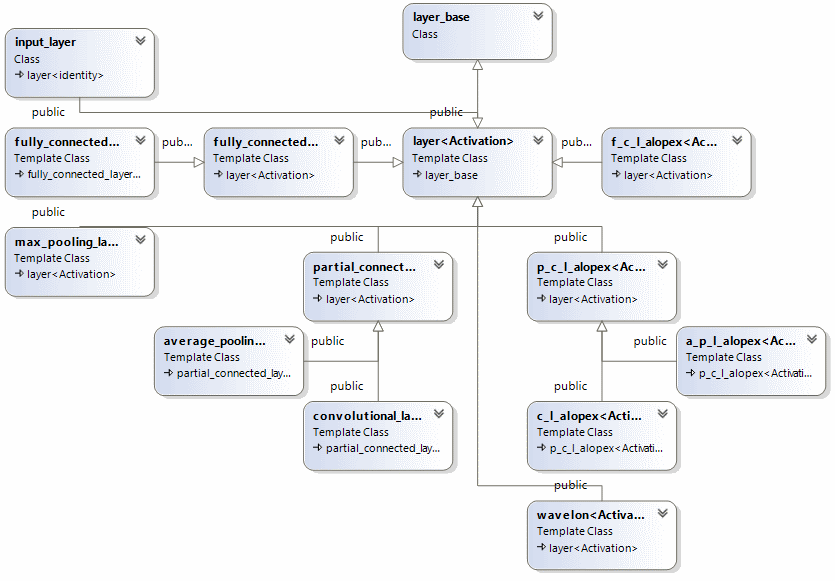
\includegraphics[width=\textwidth]{layers.png}
  }
  \caption{Диаграмма классов унаследованных от абстрактного класса слоя}\label{layers}
\end{figure}

\chapter{Тестирование результатов изменений}
В ходе тестирования стояли следующие задачи:
\begin{enumerate}
\item Проверить работоспособность используемых подходов и алгоритмов отдельно.
\item Проверить работоспособность внесенных изменений, как в первом так и во втором виде изменений.
\item В случае неработоспособности изменений локализовать проблему.
\item В случае работоспособности найти оптимальные настройки для рассматриваемого случая и сравнить результат его работы с оригинальным алгоритмом.
\end{enumerate}
\section{Набор данных MNIST}
MNIST - Mixed National Institute of Standards and Technology database. Это база содержащая рукописные цифры. В базе содержится 60000 обучающих примеров и 10000 контрольных. Использование результатов обучения по этой базе можно считать в некотором смысле стандартной процедурой для оценки результативности алгоритма. В приложении \ref{MNISTABLE} находится сводная таблица результатов разных методов, применяемых для решения задачи распознавания, на этом наборе данных. Из всей таблицы наиболее важным элементом для данной задачи является результат для сверточных нейронных сетей. Ниже приведены результаты различного использования сверточных нейронных сетей. Для каждого подхода указан процент ошибочных срабатываний.
\begin{itemize}
\item LeNet-1 : 1.7\%
\item LeNet-5 : 0.95\%
\item Группа из 35 сверточных сетей : 0.23\%
\end{itemize}

\section{Тестирование работоспособности сверточной сети реализованной в библиотеке tiny-cnn}
В ходе преддипломной практики был изучен набор библиотек, реализующих функционал сверточных нейронных сетей. В результате сравнительного анализа была выбрана библиотека tiny-cnn, как максимально отвечающая набору требований для данной работы. Для тестирования работоспособности данной библиотеки использовался набор данных MNIST с обучением пакетами по 10 изображений. На рисунке \ref{tiny_cnn_learning} приведен график обучения такой сети. После 25 эпох обучения ошибка составила 1.29\%, что вполне сопоставимо с результатом, указанным в сводной таблице результатов для этого набора данных. На основе этого можно сказать, что алгоритм, реализованный в данной библиотеке вполне работоспособен и может быть использован для дальнейшего обучения.
\begin{figure}[H]
 \centering{
 	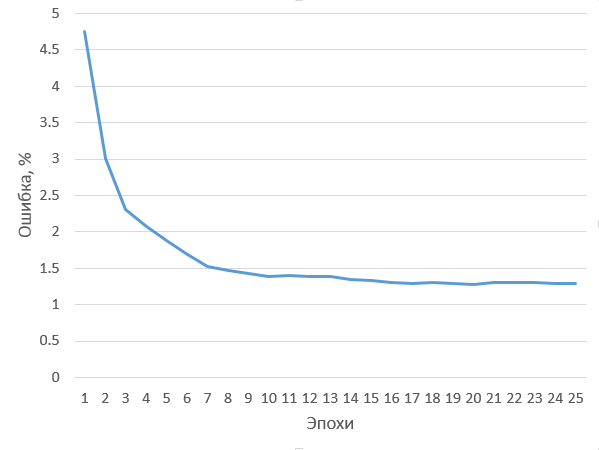
\includegraphics[width=0.9\textwidth]{tiny_cnn_learning.png}
  }
  \caption{График количества правильно распознаваемых иизображений тестовой выборки размером 10000 в зависимости от эпохи обучения}\label{tiny_cnn_learning}
\end{figure}

\section{Тестирование работоспособности алгоритма ALOPEX}
Для обучения сети в одной из модификаций требовалось использовать недифференциирующий алгоритм обучения, в качестве которого был выбран алгоритм ALOPEX. Работоспособность алгоритма тестировалась на простейших нейросетях. Для теста был взят многослойный персептрон с одним скрытым слоем, с полносвязными слоями. К нему была применена задача сложения двух чисел. При обучении параметры алгоритма подбирались для оптимизации времени обучения. Полученные результаты сходятся с упоминаемыми в работе \cite{carlo_alopex}. Из этого можно сделать вывод, что алгоритм ALOPEX реализован правильно.  На рисунке \ref{ALOPEX_test} приведен график обучения демонстрирующий зависимость ошибки от эпохи.
\begin{figure}[H]
 \centering{
 	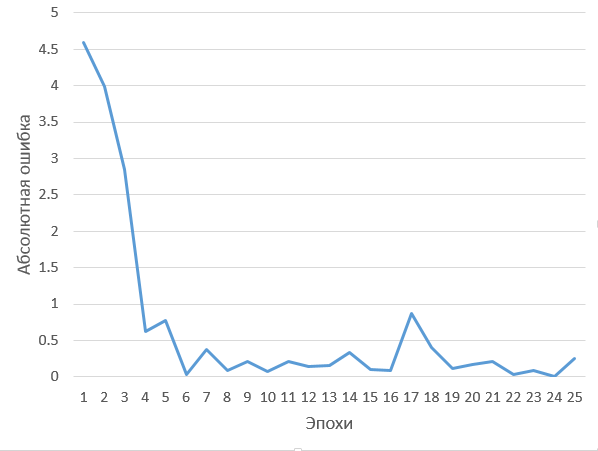
\includegraphics[width=0.9\textwidth]{ALOPEX_test.png}
  }
  \caption{График абсолютной ошибки при обучении многослойного персептрона с одним скрытым слоем по алгоритму ALOPEX}\label{ALOPEX_test}
\end{figure}

\section{Тестирование работоспособности инициализации ядра свертки набором вейвлетов}
Рассмотрим ядро свертки размером $ 5 \times 5 $, которое инициализировано нулями
Инициализируем следующие вейвлеты:
\begin{enumerate}
\item $\{X=0; Y=2; R=x; S=3; Z=0.75\}$
\item $\{X=3; Y=3; R=x; S=1; Z=-0.25\}$
\item $\{X=0; Y=0; R=y; S=4; Z=-1.0\}$
\item $\{X=4; Y=4; R=y; S=2; Z=0.75\}$
\end{enumerate}

В таком случае ядро свертки будет представлять из себя следующую матрицу:
\[ \left( \begin{array}{ccccc}
-1.0 & 1.0 & 0.0 & 0.0 & 0.0 \\
-1.0 & 1.0 & 0.0 & 0.0 & 0.0 \\
-0.25 & 1.75 & 0.75 & 0.0 & 0.0 \\
-1.75 & 0.25 & -0.75 & -0.25 & 0.0 \\
0.0 & 0.0 & 0.0 & 0.25 & 0.75 \end{array} \right)\]
Если нормировать полученную матрицу и перевести ее в графическое отображение, получится изображение приведенное на рисунке \ref{convolution_matrix}.
\begin{figure}[H]
 \centering{
 	
\includegraphics[width=0.2\textwidth]{convolution_matrix.png}
  }
  \caption{Ядро свертки, полученное в результате мысленного эксперимента}\label{convolution_matrix}
\end{figure}

Как можно видеть в результате такого метода конструирования получается корректное ядро свертки. Если инициализировать ядро такого размера большим количеством вейвлетов, то результат будет еще более похожим на обычную матрицу свертки получаемую в результате работы сверточной сети. В силу избыточности инициализации наложение различных вейвлетов может формировать паттерны не ограничивающиеся прямыми линиями параллельными осям.

\section{Тестирование практической работоспособности инициализации сверточного слоя вейвлетами}
Для практической проверки работоспособности данного изменения был применен набор данных MNIST. В алгоритм обучения, описанный в библиотеке tiny-cnn  не вносилось изменений. для теста работоспособности было выбрано количество инициирующих вейвлетов равное 10 и разброс веса  $ Z $ равный $ \pm 0.5 $. На представленных настройках сеть показала своб работоспособность. При усреднении данных 7 экспериментов результат на 7 эпохе оказался в среднем равен 9827 распознанному изображению из 10000, что дает 1,73\% ошибки распознавания. Так как этот процент распознавания близок к исходному, можно говорить о работоспособности данного метода. График прогресса обучения приведен на рисунке \ref{conwave_5_05}.
\begin{figure}[H]
 \centering{
 	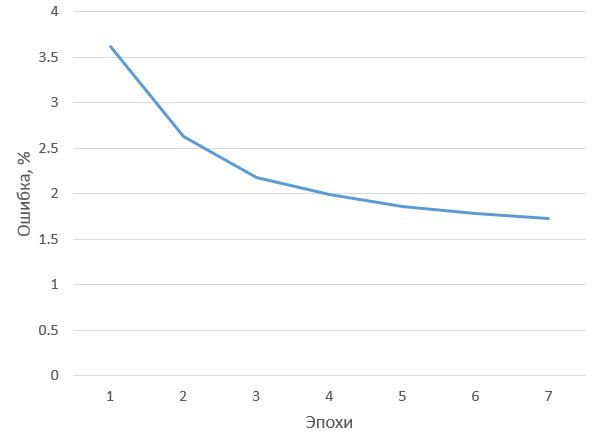
\includegraphics[width=0.9\textwidth]{conwave_5_05.png}
  }
  \caption{График обучения сети в ходе эксперимента по проверке работоспособности инциализации сверточного слоя вейвлетами}\label{conwave_5_05}
\end{figure}
На основе того, что общий вид зависимости количества распознаваемых изображений от номера эпохи не поменялся, можно сделать вывод, что данная модификация по крайней мере работоспособна.

\section{Нахождение оптимальных параметров для модификации инициализации сверточного слоя}
Так как метод инициализации сверточного слоя вейвлетами оказался работоспособен по крайней мере при некоторых параметрах встала задача подбора оптимальных параметров для такого видоизменения. Для тестов использовался набор данных MNIST. Для начала оптимизация проводилась по оси количества вейвлетов. Результаты усреднялись по 7 тестам. На графике, приведенном на рисунке \ref{conwave_different_count} кроме данных о разных результатах экспериментов приведена кривая обучения при исходной инициализации шумовыми данными (пунктирная линия). Как можно видеть для разнообразных вариантов инциализации результаты получаются в общем схожими с исходным.
\begin{figure}[H]
 \centering{
 	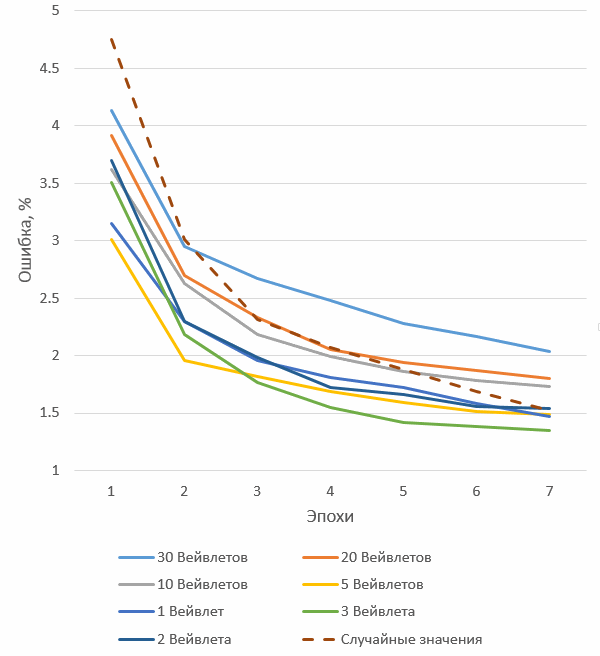
\includegraphics[width=0.9\textwidth]{conwave_different_count.png}
  }
  \caption{График зависимости количества распознаваемых изображений от эпохи по неусредненным данным от нескольких экспериментов}\label{conwave_different_count}
\end{figure}
Если после усреднения анализировать результаты на 7 эпохе для разного количества инициализирующих вейвлетов, то мы получим максимальное значение при инициализации тремя вейвлетами. Общий вид зависимости представлен на рисунке.
\begin{figure}[H]
 \centering{
 	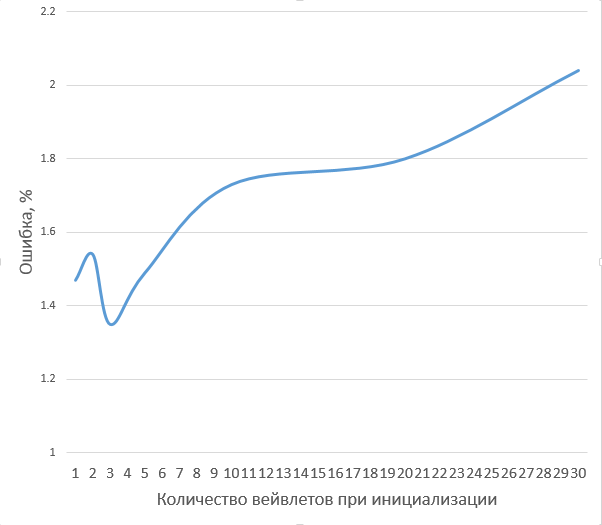
\includegraphics[width=0.9\textwidth]{conwave_different_count_oneline.png}
  }
  \caption{График зависимости количества распознаваемых изображений к седьмой эпохе от количества вейвлетов использованных при инициализации}\label{conwave_different_count_oneline}
\end{figure}
В качестве проверки граничных условий сеть была инициализирована без использования вейвлетов и шума. В данном случае сеть показала крайне медленное обучение и к концу первой эпохи имела более 90\% погрешности. Попыток инициализировать сеть более чем 30 вейвлетами не проводилось, но судя по общему виду зависимости улучшения это не принесет. Однако, добавление каждого нового вейвлета вычислительно усложняет процедуру инициализации сети.

Следующим шагом следовало выбрать параметры инициализации с точки зрения разброса коэффициента $Z$. В ходе экспериментов проводившихся аналогично поиску оптимального количества вейвлетов серьезных преимуществ параметров в окрестности $ \pm 0.5 $ обнаружено не было. Фактическая функция зависимости количества распознаных изображений на 7 эпохе от  разброса изображена на рисунке \ref{conwave_different_z_oneline}.
\begin{figure}[H]
 \centering{
 	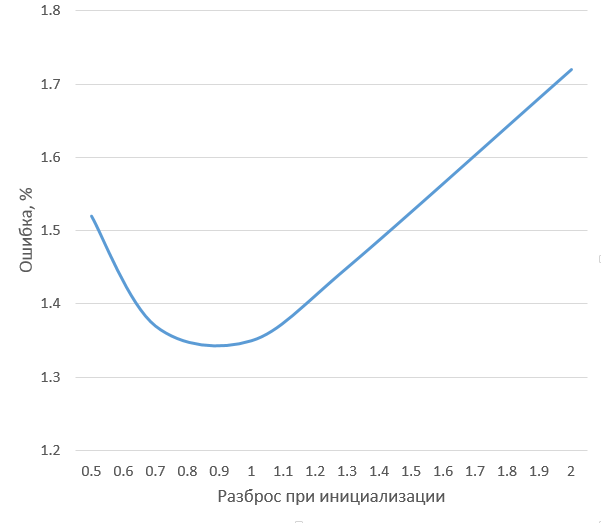
\includegraphics[width=0.9\textwidth]{conwave_different_z_oneline.png}
  }
  \caption{График зависимости количества распознаваемых изображений к седьмой эпохе от разброса коэффициента Z, использованного при инициализации}\label{conwave_different_z_oneline}
\end{figure}
Несмотря на наличие некоторого различия между этими вариантами, при просмотре неусредненных функций изображенных на рисунке \ref{conwave_different_z} можно видеть, что серьезной роли этот параметр не играет. 
\begin{figure}[H]
 \centering{
 	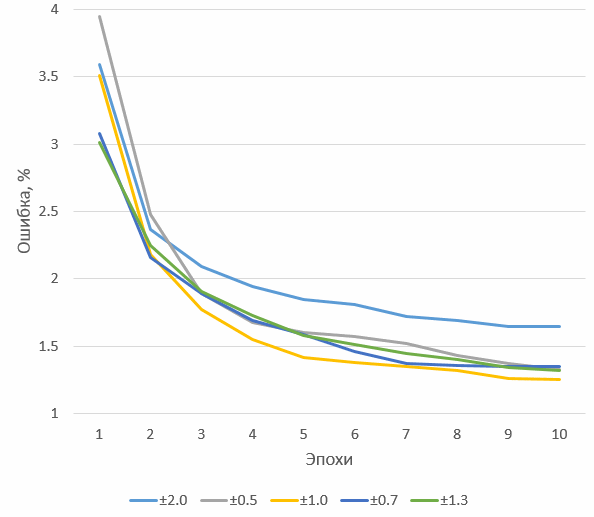
\includegraphics[width=0.9\textwidth]{conwave_different_z.png}
  }
  \caption{График зависимости количества распознаваемых изображений к седьмой эпохе от разброса коэффициента Z, использованного при инициализации}\label{conwave_different_z}
\end{figure}

\section{Проверка оптимального соотношения на возможность улучшения работы сети}
Для данного теста использовался набор данных MNIST. Данные по работе обоих вариантов работы сетей усреднялся по 5 экспериментам. Усредненные кривые обучения продемонстрированы на рисунке \ref{it_works}. Как можно видеть из приведенных графиков модификация позволяет не только начать обучение сети с более выгодной позиции, но и получить преимущество на более длительном периоде времени. В приведенном усредненном примере разница в пользу модифицированной версии составила в среднем 0.1\% ошибки. При видимой малости такого выигрыша следует заметить, что разница между наилучшими на данный момент методами перечисленными в сводной таблице составляет 0.04\% ошибки. В свою очередь эти методы так же используют сверточныей нейронные сети, правда, более сложной архитектуры.
\begin{figure}[H]
 \centering{
 	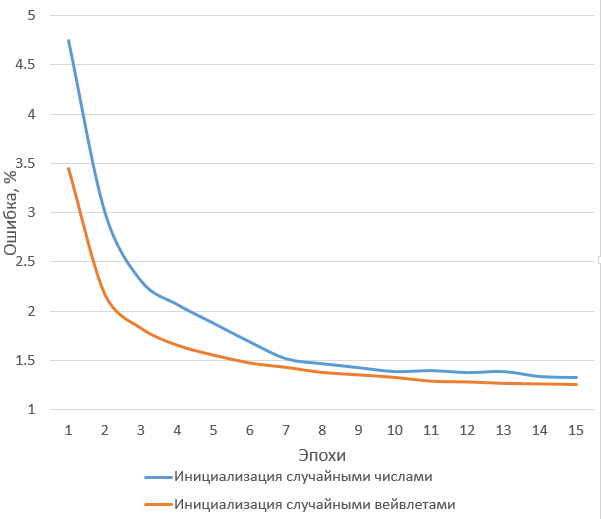
\includegraphics[width=0.9\textwidth]{it_works.png}
  }
  \caption{Сравнение графиков обучения для сверточной сети инициализированной классическим и модифицированным методами.}\label{it_works}
\end{figure}

\section{Тестирование практической работоспособности обучения сети с вейвлетами в сверточном слое}
Для данного тестового сценария каждое ядро содержало 3 вейвлета. Для алгоритма ALOPEX были выбраны следующие значения: $ \eta = 0.1; T(0) = 3.0 $. В данном случае сеть не показала способности к обучению. Количество распознаваемых ей изображений при разнообразных настройках не поднимались выше 15\% что позволяет говорить о случайном характере правильных срабатываний. После набора изменений в параметрах обучения сети признаков обучения не появилось. Таким образом эту модификацию нельзя признать рабочей. Следует разобраться в причинах неработоспособности такой модификации, или, по крайней мере обнаружить часть из них.

\section{Экспериментальное исследование проблем возникших в ходе реализации обучения сети с вейвлетами в сверточном слое}
Так как сеть инициализированная вейвлетами показала хороший результат при обучении на первых итерациях следует ожидать, что проблемы возникают в ходе работы алгоритма ALOPEX. В таком случае следует проверить зависимость качества обучения от количества настраиваемых параметров. Для этого вернемся к многослойному персептрону с одним скрытым слоем и попробуем увеличивать количество элементов в скрытом слое, тем самым увеличивая количество настраиваемых весов.
Для начала можно оценить типовые кривые обучения, для разного количества элементов в скрытом слое. На рисунках \ref{ALOPEX_sum_1}, \ref{ALOPEX_sum_2} и \ref{ALOPEX_sum_3} изображены разнообразные кривые обучения для разного количества нейронов в скрытом слое многослойного персептрона.

\begin{figure}[H]
 \centering{
 	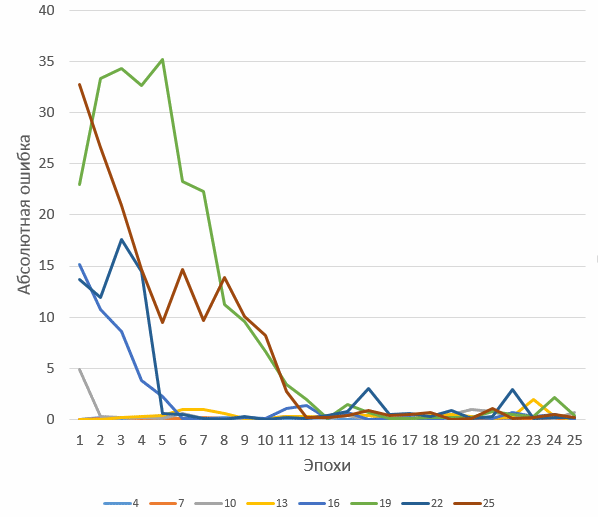
\includegraphics[width=0.8\textwidth]{ALOPEX_sum_1.png}
  }
  \caption{Кривые обучения для количества нейронов в скрытом слое меньше 50}\label{ALOPEX_sum_1}
\end{figure}
\begin{figure}[H]
 \centering{
 	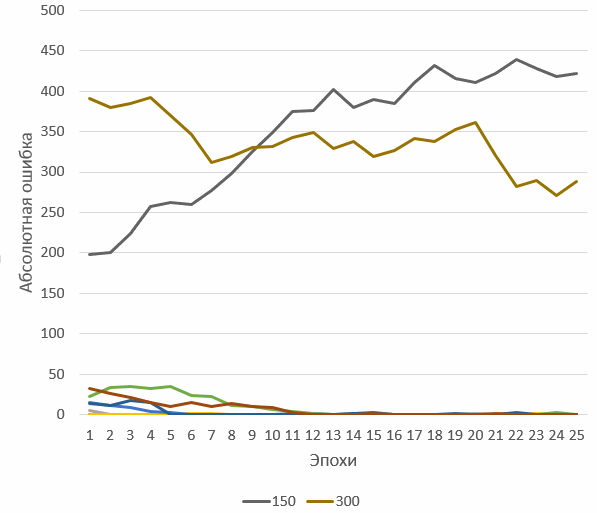
\includegraphics[width=0.8\textwidth]{ALOPEX_sum_2.png}
  }
  \caption{Дополнительно кривые обучения для 150 и 300 нейронов в скрытом слое}\label{ALOPEX_sum_2}
\end{figure}
\begin{figure}[H]
 \centering{
 	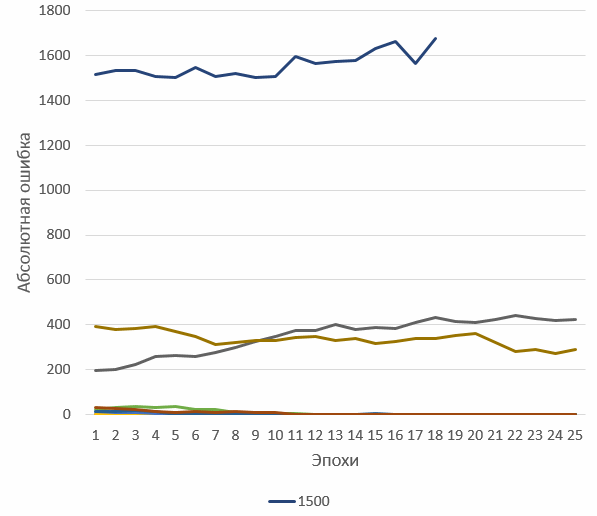
\includegraphics[width=0.8\textwidth]{ALOPEX_sum_3.png}
  }
  \caption{Дополнительно кривые обучения для 1500 нейронов в скрытом слое}\label{ALOPEX_sum_3}
\end{figure}

Переходя к более точным параметрам изучим кривую, представляющую из себя зависимость ошибки от количества нейронов в скрытом слое. Ошибка бралась минимальной за 25 эпох обучения и усреднялась за 7 экспериментов. Эта зависимость представлена на рисунке \ref{ALOPEX_errors}. В данном случае интересен не столько минимум сколько тенденция роста ошибки при увеличении количества нейронов в скрытом слое. Вкупе с предыдущими графиками это позволяет предположить, что с ростом количества настраиваемых параметров в среднем ошибка на начальных этапах заметно растет. Это позволяет предположить, что в случае со сверточными слоями, в которых количество настраиваемых превышает тысячу ошибка может быть очень серьезной, что потребует крайне длительного времени обучения, при возможности такого обучения вообще.

\begin{figure}[H]
 \centering{
 	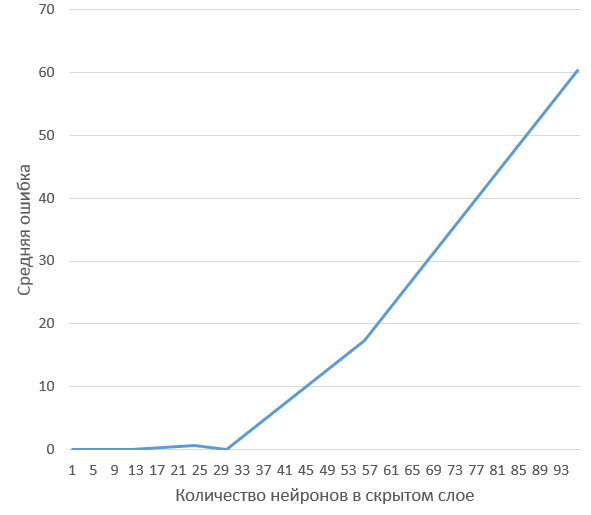
\includegraphics[width=0.9\textwidth]{ALOPEX_errors.png}
  }
  \caption{Дополнительно кривые обучения для 1500 нейронов в скрытом слое}\label{ALOPEX_errors}
\end{figure}

Если принять как обучаемость сети такой параметр как отношение максимальной ошибки за 25 эпох к минимальной за тот же период, получим следующую зависимость, изображенную на рисунке \ref{ALOPEX_learnability}. В данном случае видно, что с ростом количества настраиваемых параметров выше определенной границы обучаемость сети резко падает. Таким образом задача обучения сверточной нейронной сети при помощи алгоритма ALOPEX может оказаться просто нерешаемой или решаемой за крайне длительные сроки.

\begin{figure}[H]
 \centering{
 	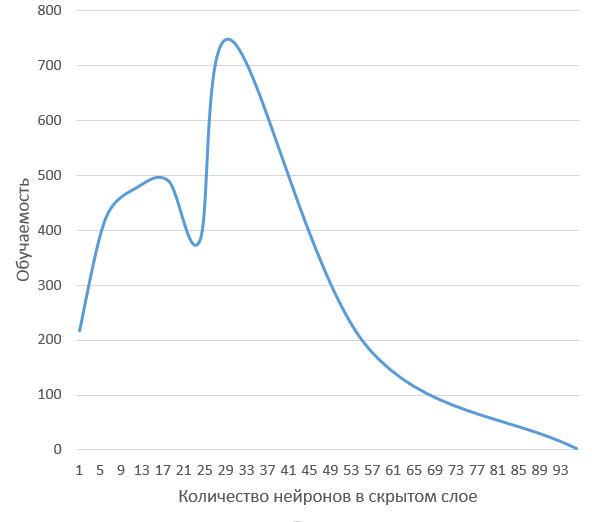
\includegraphics[width=0.9\textwidth]{ALOPEX_learnability.png}
  }
  \caption{Дополнительно кривые обучения для 1500 нейронов в скрытом слое}\label{ALOPEX_learnability}
\end{figure}

\section{Выводы на основе проведенных экспериментов}
В результате проведенного тестирования для двух вводимых модификаций были выявлены некоторые особенности. 
Модификация предполагающая инициализацию ядер свертки двумерными вейвлетами и последующее обучение сети по классическому алгоритму оказалась работоспособна, и при оптимальных настройках способна ввести не только выигрыш на начальном этапе, но и улучшить конечный результат работы сети. Безусловно это не может считаться серьезным или стабильным улучшением, так как оптимальные параметры, видимо, зависят от конкретной задачи. Однако, так как данная модификация показала устойчивое улучшение результатов на некотором количестве первых эпох можно считать ее применимой для улучшения результатов обучения в тех случаях, когда по каким-либо причинам нет возможности обучать сеть длительное количество эпох. Вероятно такая модификация работает в основном на задачах, которые подразумевают наличие на изображении именно набора линий а не пятен, которые требуется распознать, однако достоверно проверить такое предположение за время отведенное на выполнение работы не представляется выполнимым.
Модификация предполагающая изменения в алгоритме обучения оказалась неработоспособной, по крайней мере при использовании того набора средств и алгоритмов, который был опробован. Поболчным результатом экспериментов относительно этой модификации можно считать анализ работоспособности алгоритма ALOPEX, который может быть использован для построения вейвнетов произвольной размерности с недифференциируемыми активационными функциями. Что может помочь в случае с наборами данных, которые лучше аппроксимируются именно такими вейвлетами, в частности это может упростить работу с дискретными сигналами.
%% endof %

\backmatter %% Здесь заканчивается нумерованная часть документа и начинаютяс заключение и ссылки

\Conclusion % заключение к отчёту
В результате данной работы были разработаны, реализованы и испытаны две модификации сверточной нейронной сети архитектуры LeNet-5. В результате тестов можно сказать, что одна из модификаций оказалась неработоспособной, но в ходе работы над ней появились полезные побочные результаты, к которым можно отнести построение практической зависимости обучаемости многслойного персептрона с помощью алгоритма ALOPEX.
Другая модификация оказалась работоспособной и продемонстрировала снижение ошибки при работе сверточной нейронной сети на 8\%. Такая модификация применима для класса задач предполагающего наличие набора характерных линий на распознаваемом изображении. Так же эта модификация может быть использована в целях повышения скорости обучения сверточной нейронной сети на начальных эпохах обучения, так как результат работы модифицированной сети не отличается в худшую сторону от работы исходного алгоритма как в скорости сходимости, так и в итоговой точности.



\begin{thebibliography}{1} %% здесь библиографический список

\bibitem{wavelet}
{Нагорнов} О.В., {Никитаев} В.Г., {Простокишин} В.М., {Тюфлин} С.А., {Проничев} А.Н., {Бухарова} С.А., {Чистов} К.С., {Кашафутдинов} Р.З., {Хоркин} В.А.
\newblock Вейвлет анализ в примерах.
\newblock М.: НИЯУ МИФИ, 2010. – 120 с. ISBN 978-5-7262-1387-3

\bibitem{Neural_Networks}
{Комашинский} В.И., {Смирнов} Д.А.
\newblock К63 Нейронные сети и их применение в системах управления и связи.
\newblock М.: Горячая линия-Телеком, 2003. 94 c. ISBN 5-93517-094-9

\bibitem{chui}
{Чуи} Ч., {Смирнов} Д.А.
\newblock Ч87 Введение в вэйвлеты: пер. с англ.
\newblock М.: Мир, 2001. 412 c., ил

\bibitem{microsoft_paper}
{Patrice} Y.S., {Dave} S., {John} C.P.  
\newblock Best Practices for Convolutional Neural Networks Applied to Visual Documents Analysis.
\newblock Microsoft Research, Redmond, 2003

\bibitem{carlo_alopex}
{Chen} Z., {Haykin} S., {Becker} S.  
\newblock Theory of Monte Carlo sampling-based Alopex algorithms for neural networks.
\newblock Acoustics, speech, and signal processing, 1988., 2004

\bibitem{YEF}
{Abramson} Y., {Steux} B.
\newblock YEF* Real-Time Object Detection.
\newblock Ecole des Mines de Paris, Paris, 2005

\bibitem{ViolaJones}
{Viola} P., {Jones} S.M.
\newblock Robust Real-time Object Detection.
\newblock Cambridge Research Laboratory, 2001

\bibitem{alopex}
{Unnikrishnan} K.P., {Venugopal} K.P.
\newblock Alopex: A Correlation-Based Learning Algorithm for Feed-Forward and recurrent Neural Networks.
\newblock Slovenia, Ljubljana, 1994

\bibitem{LeCun}
{LeCun} Y., {Bottoy} L., {Bengio} Y., {Haffner} P.  
\newblock Gradient-Based Learning Applied to Document Recognition.
\newblock Proc. of the IEEE, November 1998

\bibitem{LM}
{Gavin} P.H.
\newblock The Levenberg-Marqardt method for nonlinear least squares curve-fitting problems.
\newblock Department of Civil and Environmental Engineering, Duke University, 2013



\end{thebibliography}

\newpage
\appendix
\appendixchapter{Сводная таблица результатов MNIST}
\label{MNISTABLE}
\begin{longtable}{p{0.3\linewidth}|p{0.2\linewidth}|p{0.1\linewidth}|p{0.2\linewidth}}
\multicolumn{4}{l}{\tablename~\ref{meer} ~Сводная таблица процентов ошибок MNIST \label{meer}}\\

classifier & preprocessing &  false rate (\%) &  Reference \\

\endfirsthead
\multicolumn{4}{l}{Продолжение таблицы~\ref{meer}}\\

classifier & preprocessing &  false rate (\%) &  Reference \\

\endhead
\multicolumn{4}{c}{Linear Classifiers} \\ \hline
linear classifier (1-layer NN) & none & 12.0 & LeCun et al. 1998 \\ 
linear classifier (1-layer NN) & deskewing & 8.4 & LeCun et al. 1998 \\
pairwise linear classifier & deskewing & 7.6 & LeCun et al. 1998  \\ 
\multicolumn{4}{c}{K-Nearest Neighbors } \\ \hline
K-nearest-neighbors, Euclidean (L2) & none & 5.0 & LeCun et al. 1998  \\ 
K-nearest-neighbors, Euclidean (L2) & none & 3.09 & Kenneth Wilder, U. Chicago  \\ 
K-nearest-neighbors, L3 & none & 2.83 & Kenneth Wilder, U. Chicago  \\ 
K-nearest-neighbors, Euclidean (L2) & deskewing & 2.4 & LeCun et al. 1998  \\ 
K-nearest-neighbors, Euclidean (L2) & deskewing, noise removal, blurring & 1.80 & Kenneth Wilder, U. Chicago  \\
K-nearest-neighbors, L3 & deskewing, noise removal, blurring & 1.73 & Kenneth Wilder, U. Chicago  \\
K-nearest-neighbors, L3 & deskewing, noise removal, blurring, 1 pixel shift & 1.33 & Kenneth Wilder, U. Chicago  \\ 
K-nearest-neighbors, L3 & deskewing, noise removal, blurring, 2 pixel shift & 1.22 & Kenneth Wilder, U. Chicago  \\ 
K-NN with non-linear deformation (IDM) & shiftable edges & 0.54 & Keysers et al. IEEE PAMI 2007  \\ 
K-NN with non-linear deformation (P2DHMDM) & shiftable edges & 0.52 & Keysers et al. IEEE PAMI 2007  \\ 
K-NN, Tangent Distance & subsampling to 16x16 pixels & 1.1 & LeCun et al. 1998  \\ 
K-NN, shape context matching & shape context feature extraction & 0.63 & Belongie et al. IEEE PAMI 2002  \\ 
\multicolumn{4}{c}{Boosted Stumps} \\ \hline
boosted stumps & none & 7.7 & Kegl et al., ICML 2009 \\ 
products of boosted stumps (3 terms) & none & 1.26 & Kegl et al., ICML 2009  \\ 
boosted trees (17 leaves) & none & 1.53 & Kegl et al., ICML 2009  \\ 
stumps on Haar features & Haar features & 1.02 & Kegl et al., ICML 2009  \\ 
product of stumps on Haar f. & Haar features & 0.87 & Kegl et al., ICML 2009 \\ 
\multicolumn{4}{c}{Non-Linear Classifiers} \\ \hline
40 PCA + quadratic classifier & none & 3.3 & LeCun et al. 1998  \\ 
1000 RBF + linear classifier & none & 3.6 & LeCun et al. 1998  \\ 
SVMs \& SVM, Gaussian Kernel & none & 1.4 &  \\ 
SVM deg 4 polynomial & deskewing & 1.1 & LeCun et al. 1998  \\ 
Reduced Set SVM deg 5 polynomial & deskewing & 1.0 & LeCun et al. 1998  \\ 
Virtual SVM deg-9 poly [distortions] & none & 0.8 & LeCun et al. 1998  \\ 
Virtual SVM, deg-9 poly, 1-pixel jittered & none & 0.68 & DeCoste and Scholkopf, MLJ 2002  \\ 
Virtual SVM, deg-9 poly, 1-pixel jittered & deskewing & 0.68 & DeCoste and Scholkopf, MLJ 2002  \\ 
Virtual SVM, deg-9 poly, 2-pixel jittered & deskewing & 0.56 & DeCoste and Scholkopf, MLJ 2002  \\ 
\multicolumn{4}{c}{Neural Nets} \\ \hline
2-layer NN, 300 hidden units, mean square error & none & 4.7 & LeCun et al. 1998  \\ 
2-layer NN, 300 HU, MSE, [distortions] & none & 3.6 & LeCun et al. 1998  \\ 
2-layer NN, 300 HU & deskewing & 1.6 & LeCun et al. 1998  \\ 
2-layer NN, 1000 hidden units & none & 4.5 & LeCun et al. 1998  \\ 
2-layer NN, 1000 HU, [distortions] & none & 3.8 & LeCun et al. 1998  \\ 
3-layer NN, 300+100 hidden units & none & 3.05 & LeCun et al. 1998  \\ 
3-layer NN, 300+100 HU [distortions] & none & 2.5 & LeCun et al. 1998  \\ 
3-layer NN, 500+150 hidden units & none & 2.95 & LeCun et al. 1998  \\ 
3-layer NN, 500+150 HU [distortions] & none & 2.45 & LeCun et al. 1998  \\ 
3-layer NN, 500+300 HU, softmax, cross entropy, weight decay & none & 1.53 & Hinton, unpublished, 2005 \\ 
2-layer NN, 800 HU, Cross-Entropy Loss & none & 1.6 & Simard et al., ICDAR 2003  \\ 
2-layer NN, 800 HU, cross-entropy [affine distortions] & none & 1.1 & Simard et al., ICDAR 2003  \\ 
2-layer NN, 800 HU, MSE [elastic distortions] & none & 0.9 & Simard et al., ICDAR 2003  \\
2-layer NN, 800 HU, cross-entropy [elastic distortions] & none & 0.7 & Simard et al., ICDAR 2003  \\ 
NN, 784-500-500-2000-30 + nearest neighbor, RBM + NCA training [no distortions] & none & 1.0 & Salakhutdinov and Hinton, AI-Stats 2007  \\ 
6-layer NN 784-2500-2000-1500-1000-500-10 (on GPU) [elastic distortions] & none & 0.35 & Ciresan et al. Neural Computation 10, 2010 and arXiv 1003.0358, 2010  \\ 
committee of 25 NN 784-800-10 [elastic distortions] & width normalization, deslanting & 0.39 & Meier et al. ICDAR 2011  \\ 
deep convex net, unsup pre-training [no distortions] & none & 0.83 & Deng et al. Interspeech 2010  \\ 
\multicolumn{4}{c}{Convolutional nets} \\ \hline
Convolutional net LeNet-1 & subsampling to 16x16 pixels & 1.7 & LeCun et al. 1998  \\ 
Convolutional net LeNet-4 & none & 1.1 & LeCun et al. 1998  \\ 
Convolutional net LeNet-4 with K-NN instead of last layer & none & 1.1 & LeCun et al. 1998  \\ 
Convolutional net LeNet-4 with local learning instead of last layer & none & 1.1 & LeCun et al. 1998  \\ 
Convolutional net LeNet-5, [no distortions] & none & 0.95 & LeCun et al. 1998  \\ 
Convolutional net LeNet-5, [huge distortions] & none & 0.85 & LeCun et al. 1998  \\ 
Convolutional net LeNet-5, [distortions] & none & 0.8 & LeCun et al. 1998  \\ 
Convolutional net Boosted LeNet-4, [distortions] & none & 0.7 & LeCun et al. 1998  \\ 
Trainable feature extractor + SVMs [no distortions] & none & 0.83 & Lauer et al., Pattern Recognition 40-6, 2007  \\ 
Trainable feature extractor + SVMs [elastic distortions] & none & 0.56 & Lauer et al., Pattern Recognition 40-6, 2007  \\ 
Trainable feature extractor + SVMs [affine distortions] & none & 0.54 & Lauer et al., Pattern Recognition 40-6, 2007  \\ 
unsupervised sparse features + SVM, [no distortions] & none & 0.59 & Labusch et al., IEEE TNN 2008 \\ 
Convolutional net, cross-entropy [affine distortions] & none & 0.6 & Simard et al., ICDAR 2003  \\ 
Convolutional net, cross-entropy [elastic distortions] & none & 0.4 & Simard et al., ICDAR 2003  \\ 
large conv. net, random features [no distortions] & none & 0.89 & Ranzato et al., CVPR 2007  \\
large conv. net, unsup features [no distortions] & none & 0.62 & Ranzato et al., CVPR 2007  \\ 
large conv. net, unsup pretraining [no distortions] & none & 0.60 & Ranzato et al., NIPS 2006  \\ 
large conv. net, unsup pretraining [elastic distortions] & none & 0.39 & Ranzato et al., NIPS 2006  \\ 
large conv. net, unsup pretraining [no distortions] & none & 0.53 & Jarrett et al., ICCV 2009 \\ 
large/deep conv. net, 1-20-40-60-80-100-120-120-10 [elastic distortions] & none & 0.35 & Ciresan et al. IJCAI 2011 \\ 
committee of 7 conv. net, 1-20-P-40-P-150-10 [elastic distortions] & width normalization & 0.27 +-0.02 & Ciresan et al. ICDAR 2011  \\ 
committee of 35 conv. net, 1-20-P-40-P-150-10 [elastic distortions] & width normalization & 0.23 & Ciresan et al. CVPR 2012  \\ 
\end{longtable}

\appendixchapter{Код инициализации ядра свертки}
%\chapter{}
%\appendixchapter{Код инициализации ядра свертки}
\label{matinit}
\begin{lstlisting}
const vec_t& forward_propagation(const vec_t& in, size_t index) override {
 if (!preconnected)
 {
  for (int i = 0; i < this->W_.size(); i++){ this->W_[i] = 0.0; }
  float_t weight;
  int x, y, length, angle;
  for (layer_size_t inc = 0; inc < in_.depth_; ++inc) {
   for (layer_size_t outc = 0; outc < out_.depth_; ++outc) {
    for (int z = 0; z < 3; z++)
    {
     static float_t quiz = 1;
     weight = static_cast <float_t> (rand()) / (static_cast <float_t> (RAND_MAX) / quiz) - quiz * 0.5; // weight
     x = rand() % window_size_;
     y = rand() % window_size_;
     length = rand() % window_size_;
     angle = rand() % 2; // vertical (0) or horizontal (1)
     if (angle == 0)
     {
      for (int w_c = 0; w_c < length; w_c++)
      {
       if ((x + w_c < window_size_) && (y + 1 < window_size_))
       {	
        this->W_[weight_.get_index(x + w_c, y, outc * in_.depth_ + inc)] += weight;	
        this->W_[weight_.get_index(x + w_c, y + 1, outc * in_.depth_ + inc)] += -weight;
       }
      }
     }
     else
     {
      for (int w_c = 0; w_c < length; w_c++)
      {
       if ((x + 1 < window_size_) && (y + w_c < window_size_))
       {
        this->W_[weight_.get_index(x, y + w_c, outc * in_.depth_ + inc)] += weight;
        this->W_[weight_.get_index(x + 1, y + w_c, outc * in_.depth_ + inc)] += -weight;
       }
      }
     }
    }
   }
  }
  preconnected = true;
 }
 return partial_connected_layer::forward_propagation(in, index);
}

\end{lstlisting}

\appendixchapter{Код абстрактного класса слоя}
%\appendixchapter{Код абстрактного класса слоя}
\label{abslayer}
\begin{lstlisting}
class layer_base {
public:
    virtual ~layer_base() {}

    layer_base(layer_size_t in_dim, layer_size_t out_dim, size_t weight_dim, size_t bias_dim) : parallelize_(true), next_(nullptr), prev_(nullptr) {
        set_size(in_dim, out_dim, weight_dim, bias_dim);
    }

    void connect(layer_base* tail) {
        if (this->out_size() != 0 && tail->in_size() != this->out_size())
            throw nn_error("dimension mismatch");
        next_ = tail;
        tail->prev_ = this;
    }

    void set_parallelize(bool parallelize) {
        parallelize_ = parallelize;
    }

    // cannot call from ctor because of pure virtual function call fan_in_size().
    // so should call this function explicitly after ctor
    void init_weight() {
        const float_t weight_base = 0.5 / std::sqrt(fan_in_size());

        uniform_rand(W_.begin(), W_.end(), -weight_base, weight_base);
        uniform_rand(b_.begin(), b_.end(), -weight_base, weight_base);               
        std::fill(Whessian_.begin(), Whessian_.end(), 0.0);
        std::fill(bhessian_.begin(), bhessian_.end(), 0.0);
        clear_diff(CNN_TASK_SIZE);
    }

    void divide_hessian(int denominator) {
        for (auto& w : Whessian_) w /= denominator;
        for (auto& b : bhessian_) b /= denominator;
    }

    // getter
    const vec_t& output(int worker_index) const { return output_[worker_index]; }
    const vec_t& delta(int worker_index) const { return prev_delta_[worker_index]; }
    vec_t& weight() { return W_; }
    vec_t& bias() { return b_; }
    vec_t& weight_diff(int index) { return dW_[index]; }
    vec_t& bias_diff(int index) { return db_[index]; }
    layer_base* next() { return next_; }
    layer_base* prev() { return prev_; }

    virtual layer_size_t in_size() const { return in_size_; }
    virtual layer_size_t out_size() const { return out_size_; }
    virtual size_t param_size() const { return W_.size() + b_.size(); }
    virtual size_t fan_in_size() const = 0;
    virtual size_t connection_size() const = 0;

    virtual void save(std::ostream& os) const {
        for (auto w : W_) os << w << " ";
        for (auto b : b_) os << b << " ";
    }

    virtual void load(std::istream& is) {
        for (auto& w : W_) is >> w;
        for (auto& b : b_) is >> b;
    }

    virtual activation::function& activation_function() = 0;
	virtual vec_t retranslations() = 0;
	virtual vec_t redilations() = 0;
    virtual const vec_t& forward_propagation(const vec_t& in, size_t worker_index) = 0;
    virtual const vec_t& back_propagation(const vec_t& current_delta, size_t worker_index) = 0;
    virtual const vec_t& back_propagation_2nd(const vec_t& current_delta2) = 0;

    // called afrer updating weight
    virtual void post_update() {}

    template <typename Optimizer>
    void update_weight(Optimizer *o, int worker_size, size_t batch_size) {
        if (W_.empty()) return;

        merge(worker_size, batch_size);

        o->update(dW_[0], Whessian_, &W_);
        o->update(db_[0], bhessian_, &b_);

        clear_diff(worker_size);
        post_update();
    }

    bool has_same_weights(const layer_base& rhs, float_t eps) const {
        if (W_.size() != rhs.W_.size() || b_.size() != rhs.b_.size())
            return false;

        for (size_t i = 0; i < W_.size(); i++)
          if (std::abs(W_[i] - rhs.W_[i]) > eps) return false;
        for (size_t i = 0; i < b_.size(); i++)
          if (std::abs(b_[i] - rhs.b_[i]) > eps) return false;

        return true;
    }

protected:
    layer_size_t in_size_;
    layer_size_t out_size_;
    bool parallelize_;

    layer_base* next_;
    layer_base* prev_;
    vec_t output_[CNN_TASK_SIZE];     // last output of current layer, set by fprop
    vec_t prev_delta_[CNN_TASK_SIZE]; // last delta of previous layer, set by bprop
    vec_t W_;          // weight vector
    vec_t b_;          // bias vector
    vec_t dW_[CNN_TASK_SIZE];
    vec_t db_[CNN_TASK_SIZE];

    vec_t Whessian_; // diagonal terms of hessian matrix
    vec_t bhessian_;
    vec_t prev_delta2_; // d^2E/da^2

private:
    void merge(size_t worker_size, size_t batch_size) {
        for (size_t i = 1; i < worker_size; i++)
            vectorize::reduce<float_t>(&dW_[i][0], dW_[i].size(), &dW_[0][0]);
        for (size_t i = 1; i < worker_size; i++)
            vectorize::reduce<float_t>(&db_[i][0], db_[i].size(), &db_[0][0]);

        std::transform(dW_[0].begin(), dW_[0].end(), dW_[0].begin(), [&](float_t x) { return x / batch_size; });
        std::transform(db_[0].begin(), db_[0].end(), db_[0].begin(), [&](float_t x) { return x / batch_size; });
    }

    void clear_diff(size_t worker_size) {
        for (size_t i = 0; i < worker_size; i++) {
            std::fill(dW_[i].begin(), dW_[i].end(), 0.0);
            std::fill(db_[i].begin(), db_[i].end(), 0.0);
        }
    }

    void set_size(layer_size_t in_dim, layer_size_t out_dim, size_t weight_dim, size_t bias_dim) {
        in_size_ = in_dim;
        out_size_ = out_dim;

        W_.resize(weight_dim);
        b_.resize(bias_dim);
        Whessian_.resize(weight_dim);
        bhessian_.resize(bias_dim);
        prev_delta2_.resize(in_dim);

        for (auto& o : output_)     o.resize(out_dim);
        for (auto& p : prev_delta_) p.resize(in_dim);
        for (auto& dw : dW_) dw.resize(weight_dim);
        for (auto& db : db_) db.resize(bias_dim);
    }

};
\end{lstlisting}



% \bibliography{biblio/filosofy} %% вместо вставки библиографии можно использовать базы BiBTeX - просто раскомментируйте эту строку.
\end{document}
